\documentclass[border=10pt]{standalone}
\PassOptionsToPackage{dvipsnames,svgnames,x11names}{xcolor}
\usepackage{tikz}
\usepackage{pgfplots}
\pgfplotsset{compat=newest}
\usepgfplotslibrary{groupplots}
\usetikzlibrary{arrows.meta}
\begin{document}
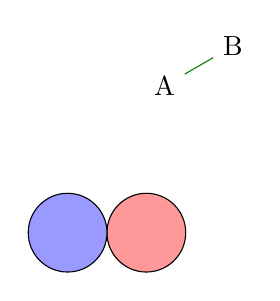
\begin{tikzpicture}
    % Define the layers library
    \pgfdeclarelayer{0}
    \pgfdeclarelayer{1}
    \pgfsetlayers{0,1}

    % Layer 0
    \begin{pgfonlayer}{0}
        \begin{scope}[rotate=30, xshift=2cm, yshift=1cm]
            \node (sa) at ({0}, {0}) {A};
            \node (sb) at ({1}, {0}) {B};
            \draw[color=green!50!black] (sa) to (sb);
        \end{scope}
        \draw[fill=red!40] ({1}, {0}) circle (0.5);
    \end{pgfonlayer}{0}

    % Layer 1
    \begin{pgfonlayer}{1}
        \draw[fill=blue!40] ({0}, {0}) circle (0.5);
    \end{pgfonlayer}{1}
\end{tikzpicture}

\end{document}
